\chapter{Architecture}
  \subsection{Choices}
    It would generate tests for test::unit, though should in theory be able to target other test frameworks with little modification.

    It would generate the tests, rather than by randomly chaining methods together, as in Randoop, by executing the program with a `mock' object that would collect data about what it was needed to be at each stage.

  \subsection{Layout}
    There's an inner core that generates the tests, an outer layer that controls it and handles file input and output, and a wrapper to pass options to the outer layer.

\begin{center}
\begin{figure}
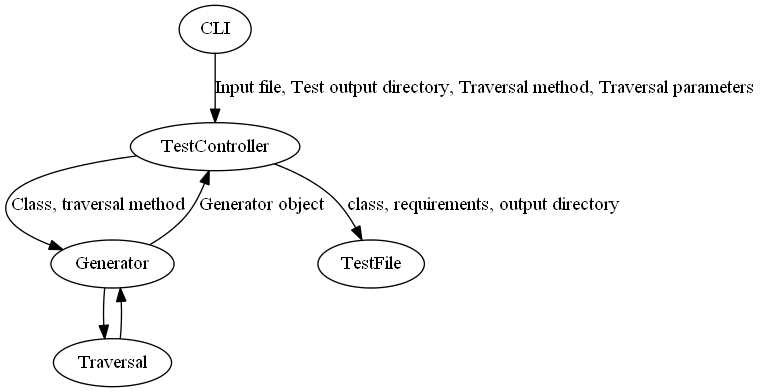
\includegraphics[width=\textwidth]{control_flow}
\caption{A short summary of the control flow of SpLATS}
\end{figure}
\end{center}
